\documentclass[a4paper,12pt]{scrartcl}
\usepackage[left= 2.5cm,right = 2cm, bottom = 4 cm, top = 2.5cm]{geometry}


% Standard Packages
\usepackage[utf8]{inputenc}
\usepackage[ngerman]{babel}
\usepackage[T1]{fontenc}
\usepackage{siunitx}
\usepackage{fancyhdr}
\usepackage{tikz}
\sisetup{detect-weight=true, detect-family=true}
\graphicspath{{img/}}
\usepackage{amsmath}
% nicht einrücken nach Absatz
\setlength{\parindent}{0pt}

% ============= Kopf- und Fußzeile =============
\pagestyle{fancy}
%
\lhead{\thepage}
\chead{}
\rhead{\slshape \leftmark}
%%
\lfoot{}
\cfoot{}
\rfoot{}
%%
\renewcommand{\headrulewidth}{0.4pt}
\renewcommand{\footrulewidth}{0pt}

\begin{document}

%\begin{center}
%\begin{tabular}{p{\textwidth}}
%

\thispagestyle{empty}

\includegraphics[scale=0.5]{img/ntb.jpg}
%
\vspace{10mm}
\begin{center}
\LARGE{\textsf{
Strömungssimulationen zur Untersuchung von Auftriebshilfen beim Leichtflugzeug FK12 Comet\\
}}
%
\vspace{1cm}
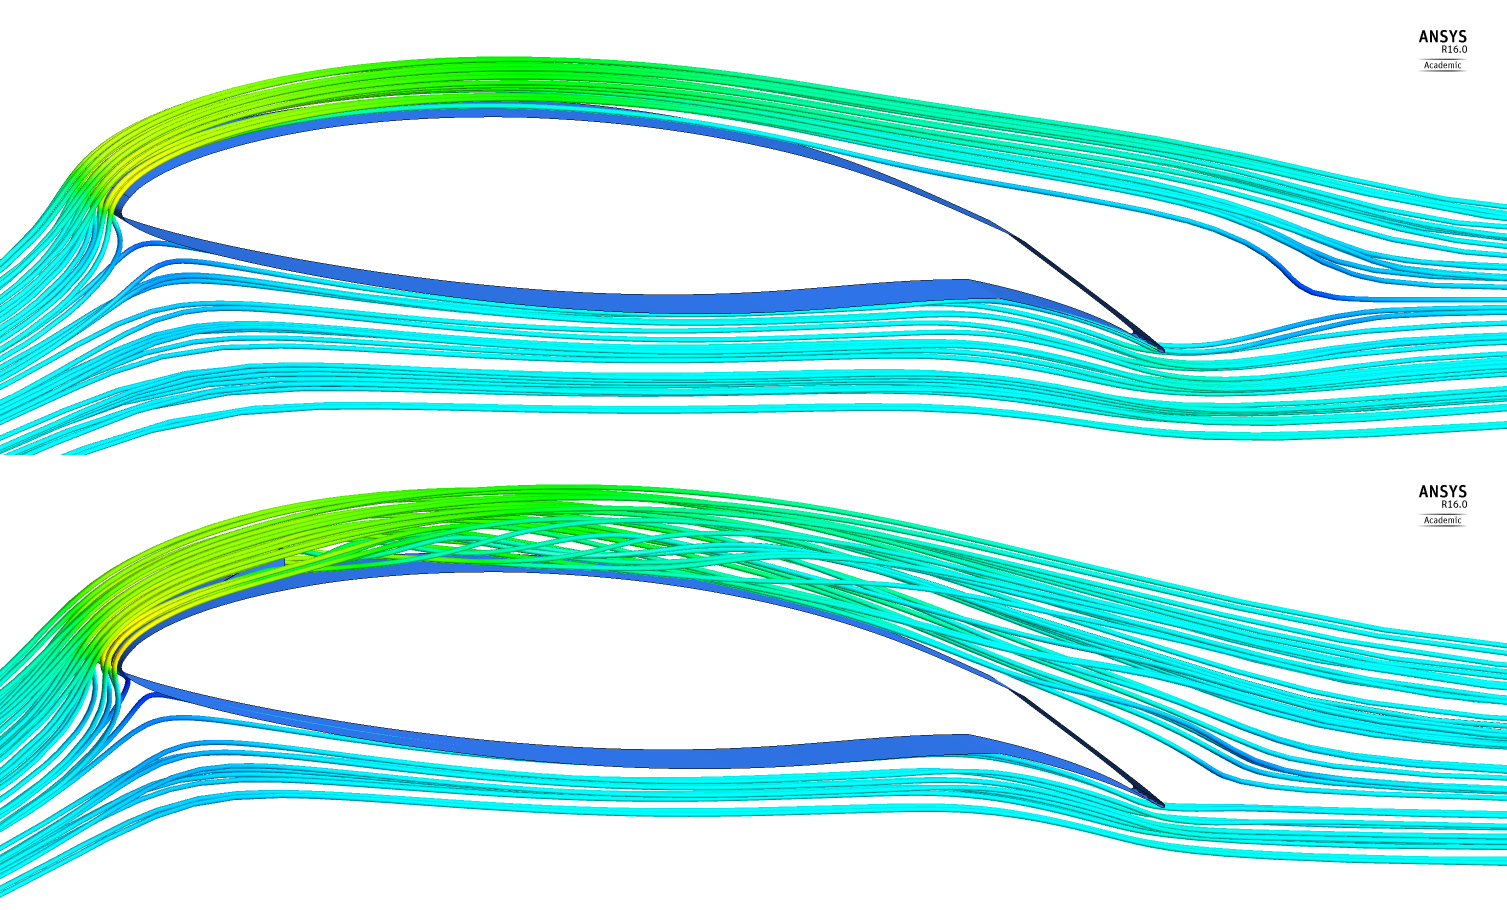
\includegraphics[width=0.99\textwidth]{titelbild_neu}
%
\end{center}
%
\begin{center}
\large{\textbf{Tim Federer und Ramon Zoller}} \\
%\small{geboren am 01.01.1900 in Musterhausen}
\end{center}
%
\vspace{2mm}
%
\begin{center}
\large{07. August 2015}
\end{center}
%
\vspace{2mm}
%\\
%
%\\
%
\begin{center}
\begin{tabular}{lll}
\textbf{Referent:} & & Prof. Dr. habil. Michael Schreiner\\
\textbf{Koreferent:} & & Prof. Dr. Christoph Würsch\\
\end{tabular}
\end{center}
%
%\end{tabular}
%\end{center}
\newpage
\pagenumbering{Roman}
\newpage
\section*{Danksagungen}
\label{danksagungen}
An dieser Stelle möchten wir all jenen danken, die durch ihre fachliche und persönliche Unterstützung zum Gelingen dieser Diplomarbeit beigetragen haben.\\
Besonderen Dank gilt Herrn Prof. Dr. habil. Michael Schreiner und Herrn Prof. Dr. Christoph Würsch für das Bereitstellen dieses interessanten Themas für die Bachelorarbeit. Zudem gaben Sie uns durch kritisches Hinterfragen immer wieder wertvolle Hinweise. Auch Ihre moralische Unterstützung und kontinuierliche Motivation haben einen grossen Teil zur Vollendung dieser Arbeit beigetragen. Sie haben uns dazu gebracht, über unsere Grenzen hinaus zu denken und zeigten uns immer wieder, wie wissenschaftliches Arbeiten abläuft. Ausserdem standen sie uns jederzeit für Fragen zur Verfügung. Vielen Dank für die Geduld und Mühen.\\

Ein weiterer Dank gilt den Mitarbeitern des ICE, die uns jeder Zeit bei der Bachelorarbeit zu verschiedenen Fragestellungen geholfen haben. Dabei geht ein besonderer Dank an Thomas Meier, Erich Carelli, Claudio Wolfer, Marco Lüchinger und Simon Härdi.
\\

Ein Dank geht auch an Peter Funk von FK-Lightplanes, welcher uns Daten zum Flugzeug, den Flügelprofilen und Fotos von den Vortexgeneratoren zur Verfügung gestellt hat.\\

Ausserdem ist ein Dank an Frau Dr. Clara Marika Velte von der technischen Universität Dänemark auszusprechen, welche uns Ihre Doktorarbeit \guillemotleft{}Characterization of Vortex Generator Induced Flow\guillemotright{} zur Verfügung gestellt hat und per E-Mail zur Verfügung stand.\\

Zusätzlich geht ein Dank an Herrn Dr. Simon Reitze, der unsere Arbeit auf Rechtschreibung und Grammatik hin korrigiert hat.\\

\begin{flushright}
Ramon Zoller und Tim Federer, im August 2015
\end{flushright}

\section*{Abstrakt}
\label{sec:abstrakt}

Die vorliegende Arbeit beschäftigt sich mit Strömungssimulationen um das Laminarflügelprofil des Flugzeugs FK12 Comet S1. Sie geht der Frage nach, wie die Flügelprofile modifiziert werden können, damit sie bessere Langsamflugeigenschaften aufweisen. 
In dieser Arbeit wird als erstes die Modifikation des Flügelprofils mit einer anderen Landeklappe betrachtet, welche beim neuen Flugzeugmodell S2 umgesetzt wurde. Die Ergebnisse zeigen den positiven Einfluss der Landeklappen auf die Langsamflugeigenschaften. Als zweites wird das Aufrüsten des Flügels S1 mit Vortexgeneratoren betrachtet. Vortexgeneratoren sind einfache geometrische Teile, welche auf der Flügeloberfläche platziert werden. Bei dieser Untersuchung wird eine Parameterstudie durchgeführt, um die Vortexgeneratoren optimal auszulegen. In den Ergebnissen ist die Wirkung deutlich zu erkennen und es können auch Rückschlüsse auf die richtige Auslegung gezogen werden. 
Die Strömungsuntersuchungen werden mit ANSYS-CFX durchgeführt; dabei ist speziell das verwendete $\gamma-Re \Theta$ Modell zu erwähnen. Dieses empirische Modell ermöglicht eine Abbildung des Umschlags von der laminaren zur turbulenten Grenzschicht.

\newpage


\section*{Abstract}
\label{sec:abstract}


The present work deals with flow simulations around the laminar airfoil of the airplane FK12 Comet S1. It examines the question, how the airfoil can be modified to improve the slow flight characteristics. 
To start, this work looked at the modification of the wingprofile with another landing flap which is in use with the new airplane model S2. The results show the positive influence of the landing flaps on the slow flight characteristics. Secondly, the upgrade of the wing profile S1 with turbulators was observed. Turbulators are simple geometrical parts that are placed on the airfoil surface. With this investigation a parameter study was performed, to lay out the turbulators optimally. The effect is clearly recognisable in the results and conclusions on the right placement can be drawn. 
The flow investigations are carried out with ANSYS-CFX; in the investigation process the $\gamma-Re \Theta$ model was used. This model allows an exact picture of the turn from the laminar to the turbulent border layer.

\newpage
\tableofcontents
\newpage
\pagenumbering{arabic}
\newpage
\pagestyle{fancy}
 \include{04_kapitel_1}

 \include{05_kapitel_2}

 \section[Algorithmen]{Algorithmen}
\label{sec:Algorithmen}
Das für einen Jouney Planner zu lösende Problem ist das Shortest-Path Problem. Un dieses Problem zu lösen gibt es mehrere Herangehensweisen. 

\subsection{Graph Basierte Algorithmen}
\label{subsec:Graph Basierte Algorithmen}
Graph-Basierte Algorithmen bilden einen Graphen aus Punkten. Die Verbindungen zwischen den Punkten werden mit einer Gewichtung versehen. Der Algorithmus iteriert nun über den Graphen und findet die Verbindung zwischen dem Start- und End-Punkt mit dem niedrigsten kombinierten Gewicht.

\subsubsection{Dijkstra}
\label{subsubsec:Dijkstra}
Der Dijkstra Algorithmus ist ein "Single-Source-Shortest-Path" Algorithmus. Er berechnet den kürzesten Weg von einem Startnode zu jedem anderen Node im Graphen. Er iteriert über alle möglichen Verbindungen und speichert das Gewicht eines Zielnodes. Wenn eine weitere Verbindung zum gleichen Node gefunden wird so wird die Verbindung mit dem geringsten Gewicht behalten. Es wird immer die Node mit dem geringsten Gewichtswert zum Startnode als nächstes berechnet. Wenn auch der Zielnode bekannt ist wird der Algorithmus gleichzeitig vom Start und Zielnode aus gestartet, so dass sie sich in der Mitte treffen. \vspace{0.5cm}

Der Dijkstra Algorithmus ist der Basisalgorithmus mit dem die anderen Algorithmen verglichen werden. Er ist konzeptionell einfach, jedoch in keiner Weise Optimiert. Die Laufzeit erhöht sich exponentiell mit der Anzahl der Nodes und Verbindungen, weshalb er für grosse Netzwerke ungeeignet ist.

\subsubsection{A*}
\label{subsubsec:A*}
Der A* Algorithmus ist eine Erweiterung des Dijkstar Algorithmus. Er sucht nicht wie der Dijkstra Algorithmus linear in alle Richtungen, sondern gezielt in Richtung des Zielnodes. Dazu wird jedem Punkt im Graph eine Entfernung zum Zielnodes zugewiesen. Nun wird dieser Wert mit dem Gewichtswert des Abstandes zum Startnode kombiniert. Der als nächstes zu berechnende Punkt wird nun aufgrund dieses Wertes entschieden. Dadurch werden Verbindungen welche in Richtung des Zieles führen präferiert un es werden viele überflüssige Rechenschritte eingespart. \vspace{0.5cm}

Obwohl der A* Algorithmus mehr Operationen pro Node durchführen muss hat er dennoch eine höhere Performance als der Dijkstra Algorithmus da viel weniger Nodes untersucht werden müssen. Der Nachteil vom A* Algorithmus ist, dass er mehr Memory benötigt.

\subsubsection{Bellman-Ford}
\label{subsubsec:Bellman-Ford}
Der Bellman-Ford Algorithmus verwendet das gleiche Grundkonzept wie der Dijkstra Algorithmus. Er achtet jedoch nicht auf den geringsten Gewichtungswert zum Startnode, sondern geht der Reihe nach alle Nodes durch. Wenn nun für einen Node nicht alle Zwischennodes zum Starnode schon berechnet wurden, so scheint dieser Node unerreichbar. Um diese Problematik zu lösen wird dieser Prozess x-1 mal wiederholt, wobei x die Anzahl der Nodes ist. \vspace{0.5cm}

Der Bellman-Ford algorithmus ist langsamer als der Dijkstra Algorithmus, da er mehrere Durchläufe über alle Nodes benötigt. Dies bietet ihm jedoch den Vorteil, dass auch eine negative Gewichtung einer Verbindung möglich ist.

\subsection{Non Graph Basierte Algorithmen}
\label{subsec:Non Graph Basierte Algorithmen}
In diesem Abschnitt werden Algorithmen erläutert, welche nicht auf das Grundkonzept des Dijkstra Algorithmus aufbauen.

\subsubsection{RAPTOR}
\label{subsubsec:RAPTOR}
Der Round-Based Public Transit Routing Algorithmus, auch RAPTOR Algorithmus genannt, ist eine Rundenbasierter, auf öffentliche Verkehrsnetzwerke zugeschnittener Algorithmus welcher auf die vorgegebenen Zuglinien achtet. \vspace{0.5cm}

Der RAPTOR Algorithmus durchläuft mehrere Runden um von der Startstation zur Zielstation zu finden. in der ersten Runden werden alle Zuglinien gescannt, welche durch die Startstation verlaufen. Wenn eine andere Zuglinie die gescannte Zuglinie Kreuzt so wird die andere Zuglinie sowei die Kreuzungsstation markiert. In der nächsten Runde werden nun alle markierten Zuglinien gescannt. Dieser Prozess wird so lange Weitergeführt, bis sich die Zielstation in einer gescannten Zuglinie befindet. Nun kann anhand der Kreuzungsstationen die Route erstellt werden. \vspace{0.5cm}

Der RAPTOR Algorithmus hat besitzt eine höhere Performanz als alle Graph Basierten Algorithmen.

\subsubsection{Connection Scan Algorithm}
\label{subsubsec:Connection Scan Algorithm}
Der Connection Scan Algorithm, kurz CSA, ist schon vom Grundkonzept auf Zeitplanbasierte Netzwerke zugeschnitten. Er arbeitet mit Stations, Connections, Trips und Footpaths. Eine Connection ist die Verbindung zwischen zwei Stationen während ein Trip den gesamten Weg eines Zuges darstellt. \vspace{0.5cm}

In einem Ersten Schritt werden die Daten in die benötigte Timetable-Form gebracht und alle Connections nach der Abfahrtszeit sortiert. Diese Schritte werden preprocessed. Danach wird über alle Connections iteriert. Eine Connection wird als erreichbar markiert, wenn sie an bereits als erreichbar Markierte Connections anschliesst oder mit der Startstation verbunden ist. Dies wird dann solange durchgeführt bis die Zielstation erreicht ist. Anschliessend wird von der Zielstation aus der verfolgte Weg zusammengesetzt, so dass ein Journey von der Startstation zur Zielstation entsteht. \vspace{0.5cm}

Für grosse Netzwerke kann der CSA mit eine Quadtree-Preprocessing schritt erweitert werden. Dabei wird das Netzwerk in immer kleiner werdende Quadrate unterteilt. Für Quadrate welche nicht die Start- oder Zielstation enthalten müssen nun nur noch die Connections beachtet werden, welche über die Ränder des Quadrates hinaus gehen. Somit können für Fernverbindungen die Lokalen Connections ignoriert werden. \vspace{0.5cm}

Im gegensatz zum Dijkstra müssen beim CSA die Connections nicht nach dem nächsten Schritt durchsucht werden, da die Abfolge durch die Preprocessing-Schritte schon definiert wurde. Dies führt zu einer Performanceverbesserung im mehrstelligen Bereich. Ein Nachteil ist jedoch, dass Preprocessing-Schritte von nöten sind und so nicht in echtzeit auf Verspätungen reagiert werden kann. Da diese Schritte jedoch nur wenige Sekunden benötigen ist dies kein schwerwiegender Nachteil. Mit der Erweiterung des Quadtree-Preprocessings können auch Anfragen in landesweite Netzwerke in wenigen Millisekunden berechnet werden. 

Im Vergleich zum RAPTOR Algorithmus bietet der CSA eine höhere Performance.


\subsection{Transfer Pattern}
\label{subsec:Transfer Pattern}
Transfer Pattern ist eine Algorithmusstrategie welche auf Preprocessing setzt. Alle möglichen Verbindungen werden mithilfe eines der zuvor genannten Algorithmen berechnet und in einem Datensatz gespeichert. Die eigentliche Anfrage beschränkt sich dann auf eine Query-Abfrage auf diesen Datensatz. \vspace{0.5cm}

Um das Preprocessing zu beschleunigen können mehrere Erweiterungen hinzugefügt werden. Eine davon ist die Verwendung von Hubs. Dabei werden die grössten Stationen als Hubs markiert. Zwischen diesen Hubs werden alle Transfer Pattern berechnet. Bei Stationen welche keine Hubs sind werden nur die Verbindungen bis zum nächsten Hub berechnet. Sollte nach drei Zugwechseln kein Hub erreicht sein so wird die Verbindung verworfen. Dies kann zwar zu Fehlern führen, ist aber vernachlässigbar, da die Fehlerrate laut Experimenten bei drei Promill liegt. \vspace{0.5cm}

Der Preprocessing kann je nach Grösse und Struktur des Netzwerks eine lange Zeit in Anspruch nehmen. Selbst mit allen Erweiterungen braucht das Preprocessing für das CH-Netzwerk vier Stunden. Dafür benötigen die Query-Anfragen nur wenige Millisekunden. Der Nachteil ist jedoch, dass mit Transfer Pattern nicht auf Zugverspätungen und Fahrplanänderungen reagiert werden kann. 





\include{07_kapitel_4}

\include{08_kapitel_5}

\include{09_kapitel_6}

\newpage
\listoffigures
	\bibliography{test2,Programme}
	\bibliographystyle{IEEEtran}

\thispagestyle{empty}
\section*{Eidesstattliche Erklärung}
%\addsec{Eidesstattliche Erklärung}
\label{sec:erklaerung}

Hiermit versichern wir, die vorliegende Arbeit selbstständig und nur unter Verwendung der von uns angegebenen Quellen und Hilfsmittel verfasst zu haben. Sowohl inhaltlich als auch wörtlich entnommene Inhalte wurden als solche kenntlich gemacht. Die Arbeit hat in dieser oder vergleichbarer Form noch keinem anderem Prüfungsgremium vorgelegen. \\
\\[1.5cm]
Datum:	\hrulefill\enspace Unterschrift: \hrulefill
\\
\begin{flushright}
\large Dr. No \\[1.5cm]
\end{flushright}

Datum:	\hrulefill\enspace Unterschrift: \hrulefill \\
\begin{flushright}
\large Goldfinger \\[1.5cm]
\end{flushright}


\end{document}
